

\begin{table}
    \centering
    \caption{Parameters of the second shaker test.}
    \label{tab:shaker_param_02}
    \begin{tabular}{cccccccc} 
    \toprule
    \multicolumn{5}{c}{\textbf{Harmonic frequency} {[}Hz]} & \multirow{2}{*}{\textbf{Amplitude }{[}mV\_\{pp\}]} & \multicolumn{2}{c}{\textbf{ No. of snapshots}} \\
    10 & 30 & 60 & 70 & 100 &  & Train & Test \\ 
    \hline
    - & 0.1 & - & 1.0 & 1.0 & 580 & 100 & 10 \\
    - & 0.1 & - & 1.0 & 1.0 & 1000 & 100 & 10 \\
    - & 0.1 & - & 1.0 & 1.0 & 1980 & 100 & 10 \\
    - & 0.1 & - & 1.0 & 1.0 & 1540 & 100 & 10 \\
    - & 0.1 & - & 1.0 & 1.0 & 2000 & - & 20 \\
    - & 0.1 & - & 1.0 & 1.0 & 0 & - & 10 \\
    - & 0.1 & - & 1.0 & 1.0 & 800 & - & 10 \\
    - & 0.1 & - & 1.0 & 1.0 & 200 & - & 10 \\
    - & 0.1 & - & 1.0 & 1.0 & 1220 & - & 10 \\
    1.0 & 1.0 & 0.1 & - & - & 1540 & - & 10 \\
    \bottomrule
    \end{tabular}
    \end{table}

\begin{figure}
    \centering
    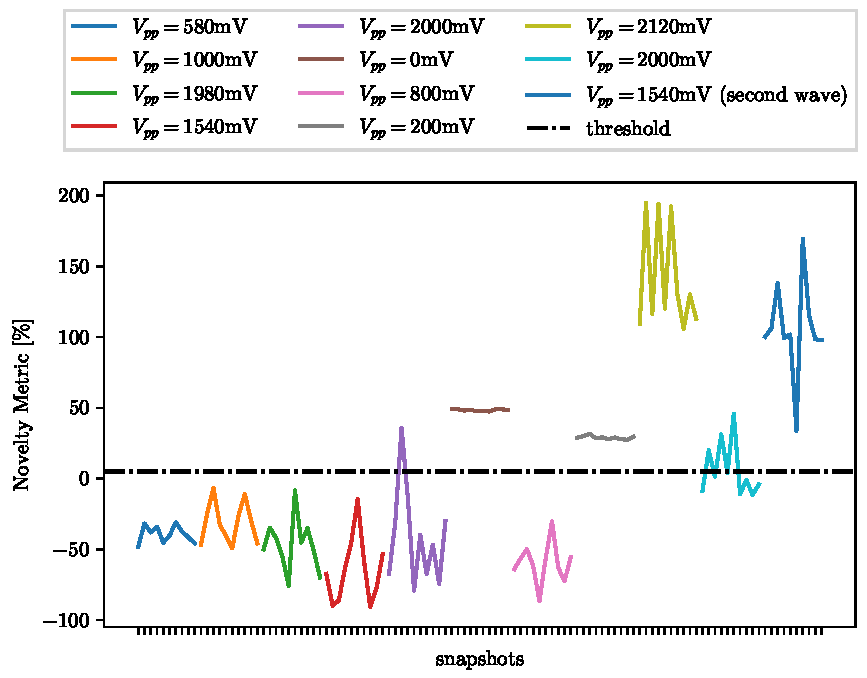
\includegraphics{Images/shaker/Test02.pdf}
    \caption{Novelty detection result}
    \label{fig:shaker_results02}
\end{figure}

\begin{figure}
    \centering
    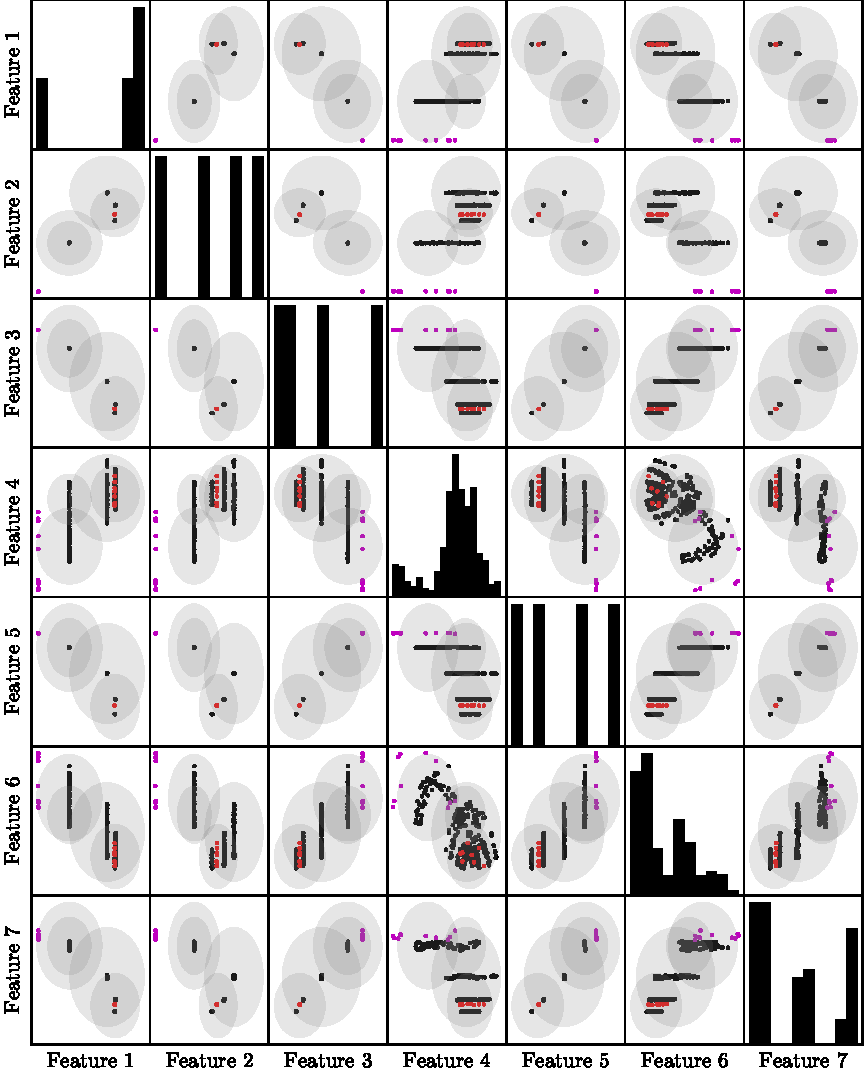
\includegraphics{Images/shaker/ConfusionMatrix.pdf}
    \caption{False Negative and True Positive results. On the diagonal, there is an histogram of the feature values. The off-diagonal plots are the scatter plots of the features. The shades are the projection of the clusters on the considered plane. (Red: False Negative, Magenta: True Positive, Black: training data)}
    \label{fig:shaker_conf_matrix}
    \end{figure}